%\documentclass[11pt,twoside]{mitthesis}
%\usepackage{tikz}
%\usepackage{circuitikz}
%\usepackage{amsmath}
%\newcommand{\ohm}{$\Omega$ }
%\begin{document}
\chapter{Hardware}


Block diagram / Schematic


\begin{figure}[h]
  \begin{center}
      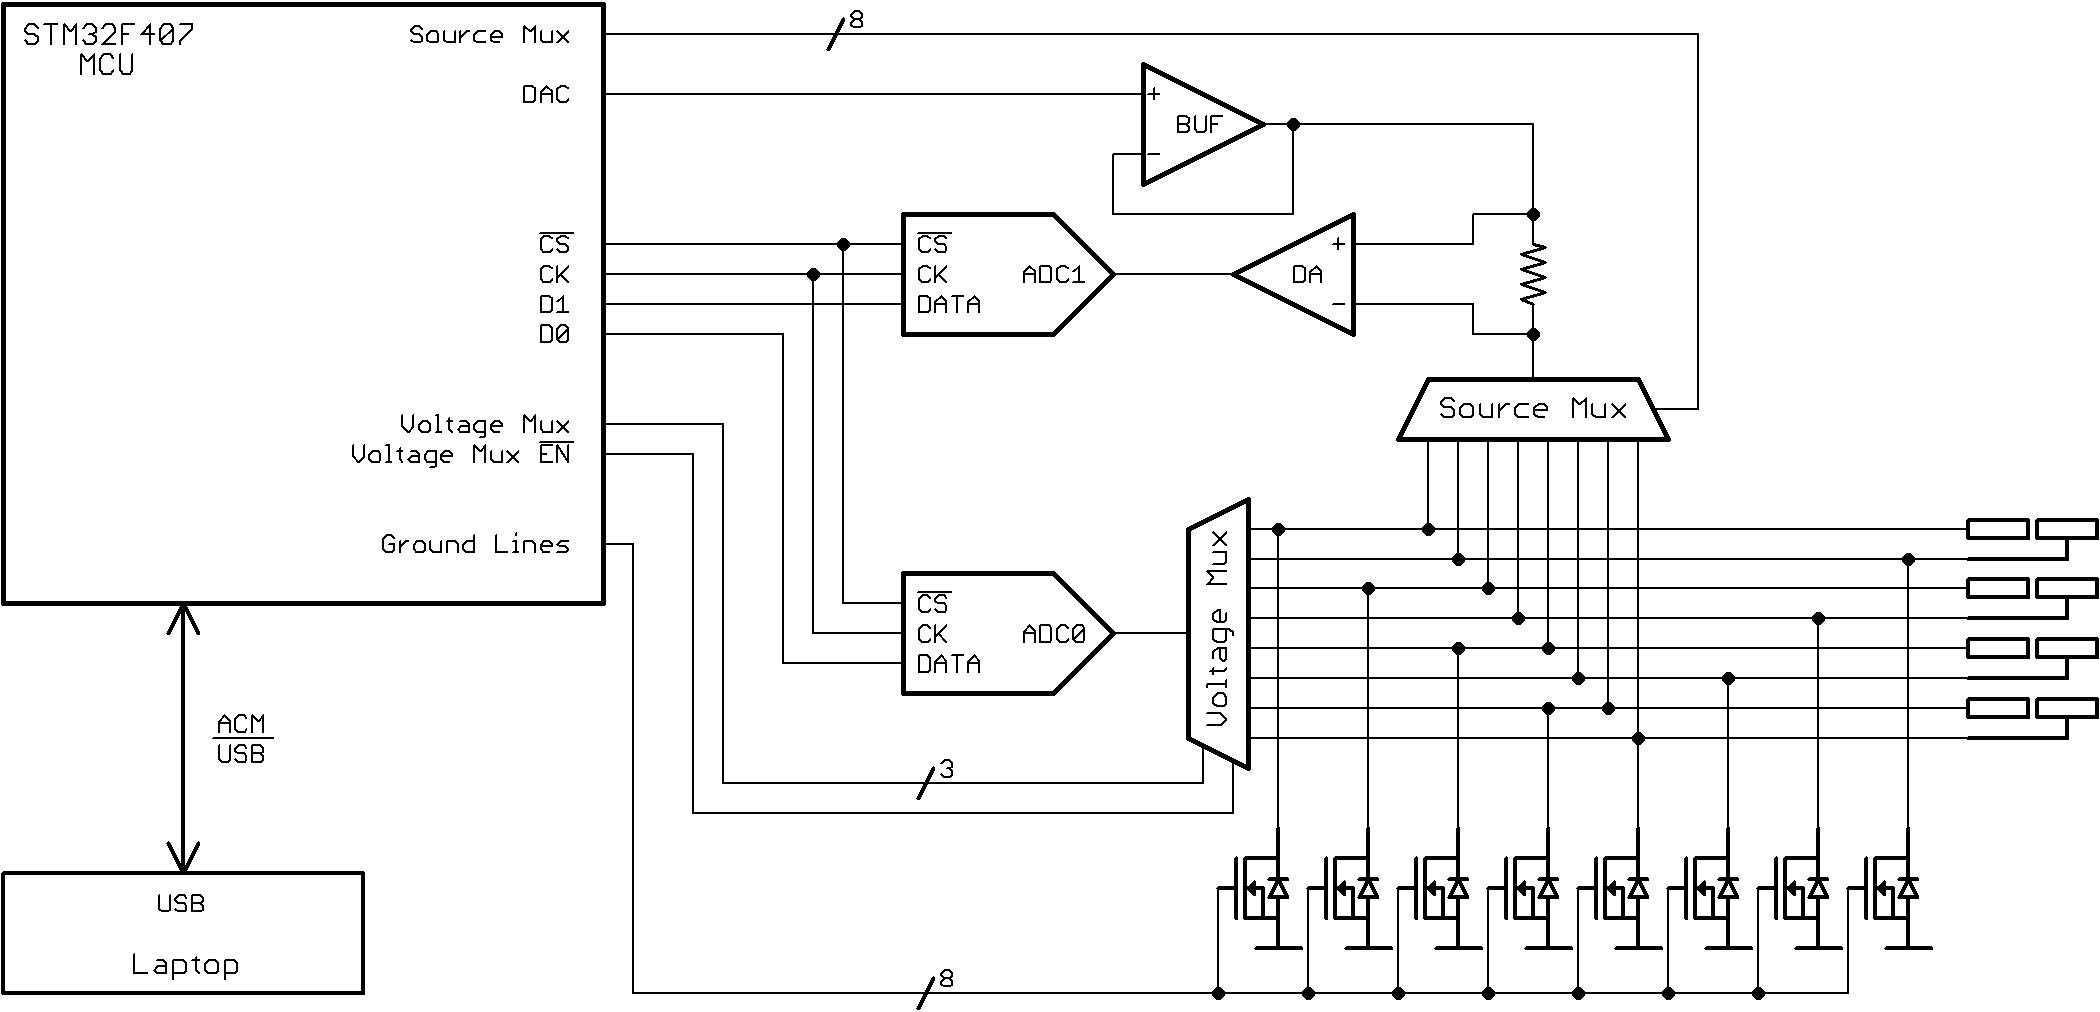
\includegraphics[width=1\textwidth]{../circuit.png}
  \end{center}
\end{figure}
\section{Low Cost}

Keeping the cost of production low makes butterboard accessible to the largest population of people.
Using multiplexed ADCs where possible keeps the cost down by reducing the quantity of high price-tag components, like ADCs.

\section{Node Voltage Reading}

Although the STM32F407 has three onboard 12-bit A/D converters, their specifications are lacking.
Each is able to sample at 2MSPS, and it's possible to interleave them to attain a sampling rate of 6MSPS or higher if you're willing to throw away bits.
The total unadjusted error (offset error, gain error, differential linearity error, and integral linearity error) is between $\pm$2 LSB and $\pm$5 LSB.
With a minimum of $\pm$2 LSB's of error, the lowest significant two bits in the 12-bit A/D are virtually useless.
Another specification to consider is the input circuitry to the ADC.
The input circuitry to the ADC while it's in tracking mode looks like a 6K$\Omega$ resistor charging a 4pF capacitor.
This puts a pole at 6.6MHz, causing .3\% error in measurement at 100KHz, 3\% error in measurement at 1MHz, and 7\% at 3MHz.
When sampling at the maximum sample rate of 6MSPS, the ADC's input network begins to introduce significant error.
Granted, it's likely that there will be an alternative bandwidth bottleneck, this is still a metric of concern.
[DM00037051.pdf, pages 133-134]

An ADCS7476 12-bit A/D converter is used to measure the voltages at each node.
The ADCS7476 can sample up to 1MSPS with $\pm$1 LSB of total unadjusted error from $-40^o C$ to $85^o C$ and $<\pm 0.2$ LSB of error at $25^o C$.
No bits are wasted in the ADCS7476 A/D converter.
Additionally, the input circuitry to the ADC is a 100$\Omega$ resistor in series with a 26pF capacitor.  
This places a pole at 61MHz, causing a .03\% error at 100KHz and .3\% error at 1MHz.
The additional performance is well worth the additional cost of \$1.56375 in quantities of 1Ku.

The ADC is connected to the common pin of a CD4051 1:8 analog multiplexer.
The multiplexer is connected to eight breadboard rails, which allows the ADC to measure the voltage on any of the eight rails, one rail at a time.

The CD4051 has about $200\Omega$ of series resistance and 30pF of output capacitance when its supply voltage is 12V, which places an additional pole at 26MHz, again well above the Nyquist frequency.

So far, the voltage-reading signal chain has two poles - one at 61MHz and one at 26MHz.

\section{Signal Generator}

The STM32F407 has an onboard D/A converter that is good enough to use as a signal generator.
The onboard DAC is configured to output a cosine wavetable with a DC offset, as described in the next chapter.

\section{Test Voltage Current Sensing}

The DAC output is buffered by half of an MCP6L92 10MHz op-amp.
The onboard DAC can be configured with an optional onboard buffer, but the buffer limits the DAC output range from 0.2V to Vdd-0.2V.
Without the onboard buffer, the DAC output is 15k$\Omega$.
When configured as a voltage buffer, the MCP6L92 has an input impedance larger than 1G$\Omega$, resulting in no signal attenuation.

\begin{figure}[h!]
  \begin{center}
      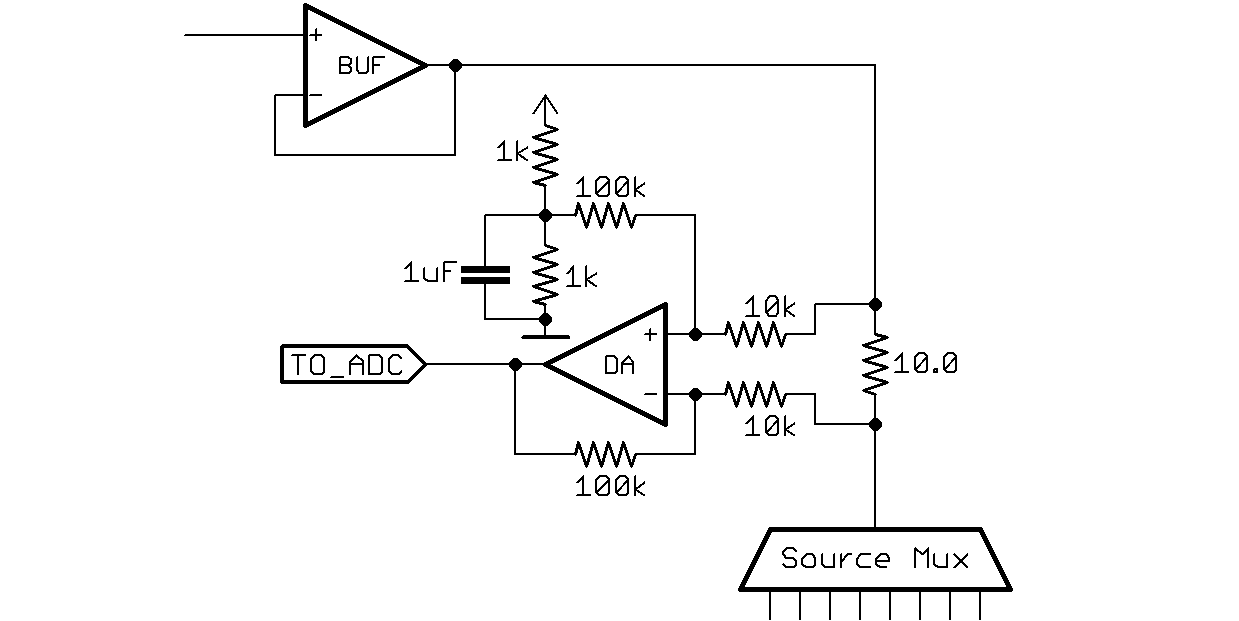
\includegraphics[width=.7\textwidth]{../DA.png}
      \caption{Difference Amplifier Schematic}
  \end{center}
\end{figure}

The buffer sources current through a 10.0\ohm, 1\% sense resistor, which can be switched onto any of the breadboard rails through an array of eight high-side switches.
The voltage across the sense resistor is measured by the other half of the MCP6L92 op-amp configured as a simple difference amplifier.
Using two 10k\ohm resistors and two 100k\ohm resistors, the difference amplifier is configured with a gain of 10.  

\begin{figure}[h!]
  \begin{center}
      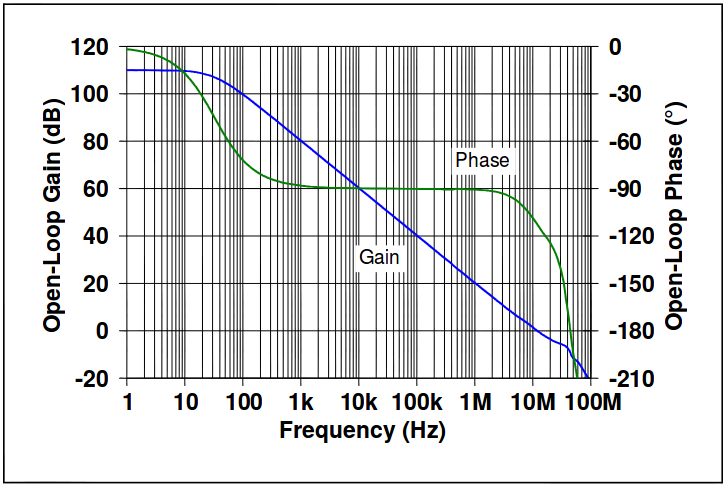
\includegraphics[width=.6\textwidth]{../opamp-bode.png}
      \caption{MCP6L92 Open Loop Bode Plot}
  \end{center}
\end{figure}

According to the MCP6L92 datasheet, the difference amplifier should have a -3dB bandwidth of 1MHz and plenty of phase margin driving the 100\ohm - 26pF input impedance to the current sense ADC.

\newpage
\section{High-side Switches}

The high-side switches were selected for high-voltage operation, so that any rail of the breadboard could swing between 0 and 30V and there wouldn't be a problem.
The selected switches were Vishay DG468 normally open analog switches.
They have 9\ohm resistance and 76pF of capacitance in the on-state, 1nA of leakage current and 30pF of capacitance in the off-state.
The high and low side switches are the main limits of bandwidth due to their high amounts of input capacitance in both on and off states.


\section{Low-side Switches}

The low-side switches have a low logic-level threshold voltage, low drain-source on-resistance, can handle up to 30V, and are low-cost.
The IRLML2803 N-FETs have an $R_{DS_{ON}}$ of about 1\ohm with a $V_{GS}$ of 3.3V.
With 10V $V_{GS}$, $R_{DS_{ON}}$ drops to 250m\ohm.


HIGH $C_{DS}$.

\section{PCB Mounted Breadboard}

\section{Hardware Prototypes}
%\end{document}
